\documentclass[a4paper,10pt]{article}
\usepackage{graphicx,color}
\usepackage[margin=2cm]{geometry}
\usepackage{algorithm2e}

\begin{document}

{\LARGE{\centerline{\bf Lab 1}}}

\section{Matrix Addition}
Matrix addition is completed element wise. To calculate an element in matrix $C$, the corresponding elements in both matrix $A$ and matrix $B$ are added. Two dimentional and three dimentional addition are accomplished in the same manner.
\begin{equation}
	c_{ij} = a_{ij}+b_{ij}
\end{equation}
\begin{equation}
	c_{ijk} = a_{ijk}+b_{ijk}
\end{equation}
This was accomplished by using nested \texttt{for} loops. While this method is inefficient, it is simple and is easily parallelisable.


\section{Matrix Multiplication}

Matrix $C$ is the result of multiplying matrix $A$ and $B$.
In two dimensions, both $A$ and $B$ are square matrices of equal size, $N$.
In three dimensions, both $A$ and $B$ are cubic matrices of equl size, $N$.
The matrices $A$ and $B$ are populated with random values that range $0 - 20$.
$N$ is set to 10 and 20.

\subsection{Two Dimensional Matrices}

Each element in matric $C$ is found using equation \ref{2Dmult}.

\begin{equation}\label{2Dmult}
c_{i,j}=\sum_{k} a_{i,k} \times b_{k,j}
\end{equation}

This is achieved using three seperate \texttt{for} loops.
The first \texttt{for} loop traverses the rows of $C$, while the second \texttt{for} loop traverses the columns.
The third \texttt{for} loop traverses the row and column of matrices $A$ and $B$.

\subsection{Three Dimensional Matrices}

To obtain each element in matrix $C$, matrix $A$ and $B$ are divided into two dimensional matrices, $A'$ and $B'$ as can be seen in figure \ref{3DMult}.
For each two dimensional matrix, a single row and column is multiplied to get the corresonding element in the $C$ matrix.
This leads to a single value which is the element in the $C$ matrix.
This is done for all elements in the $C$ matrix.

\begin{figure}[h]
\centering
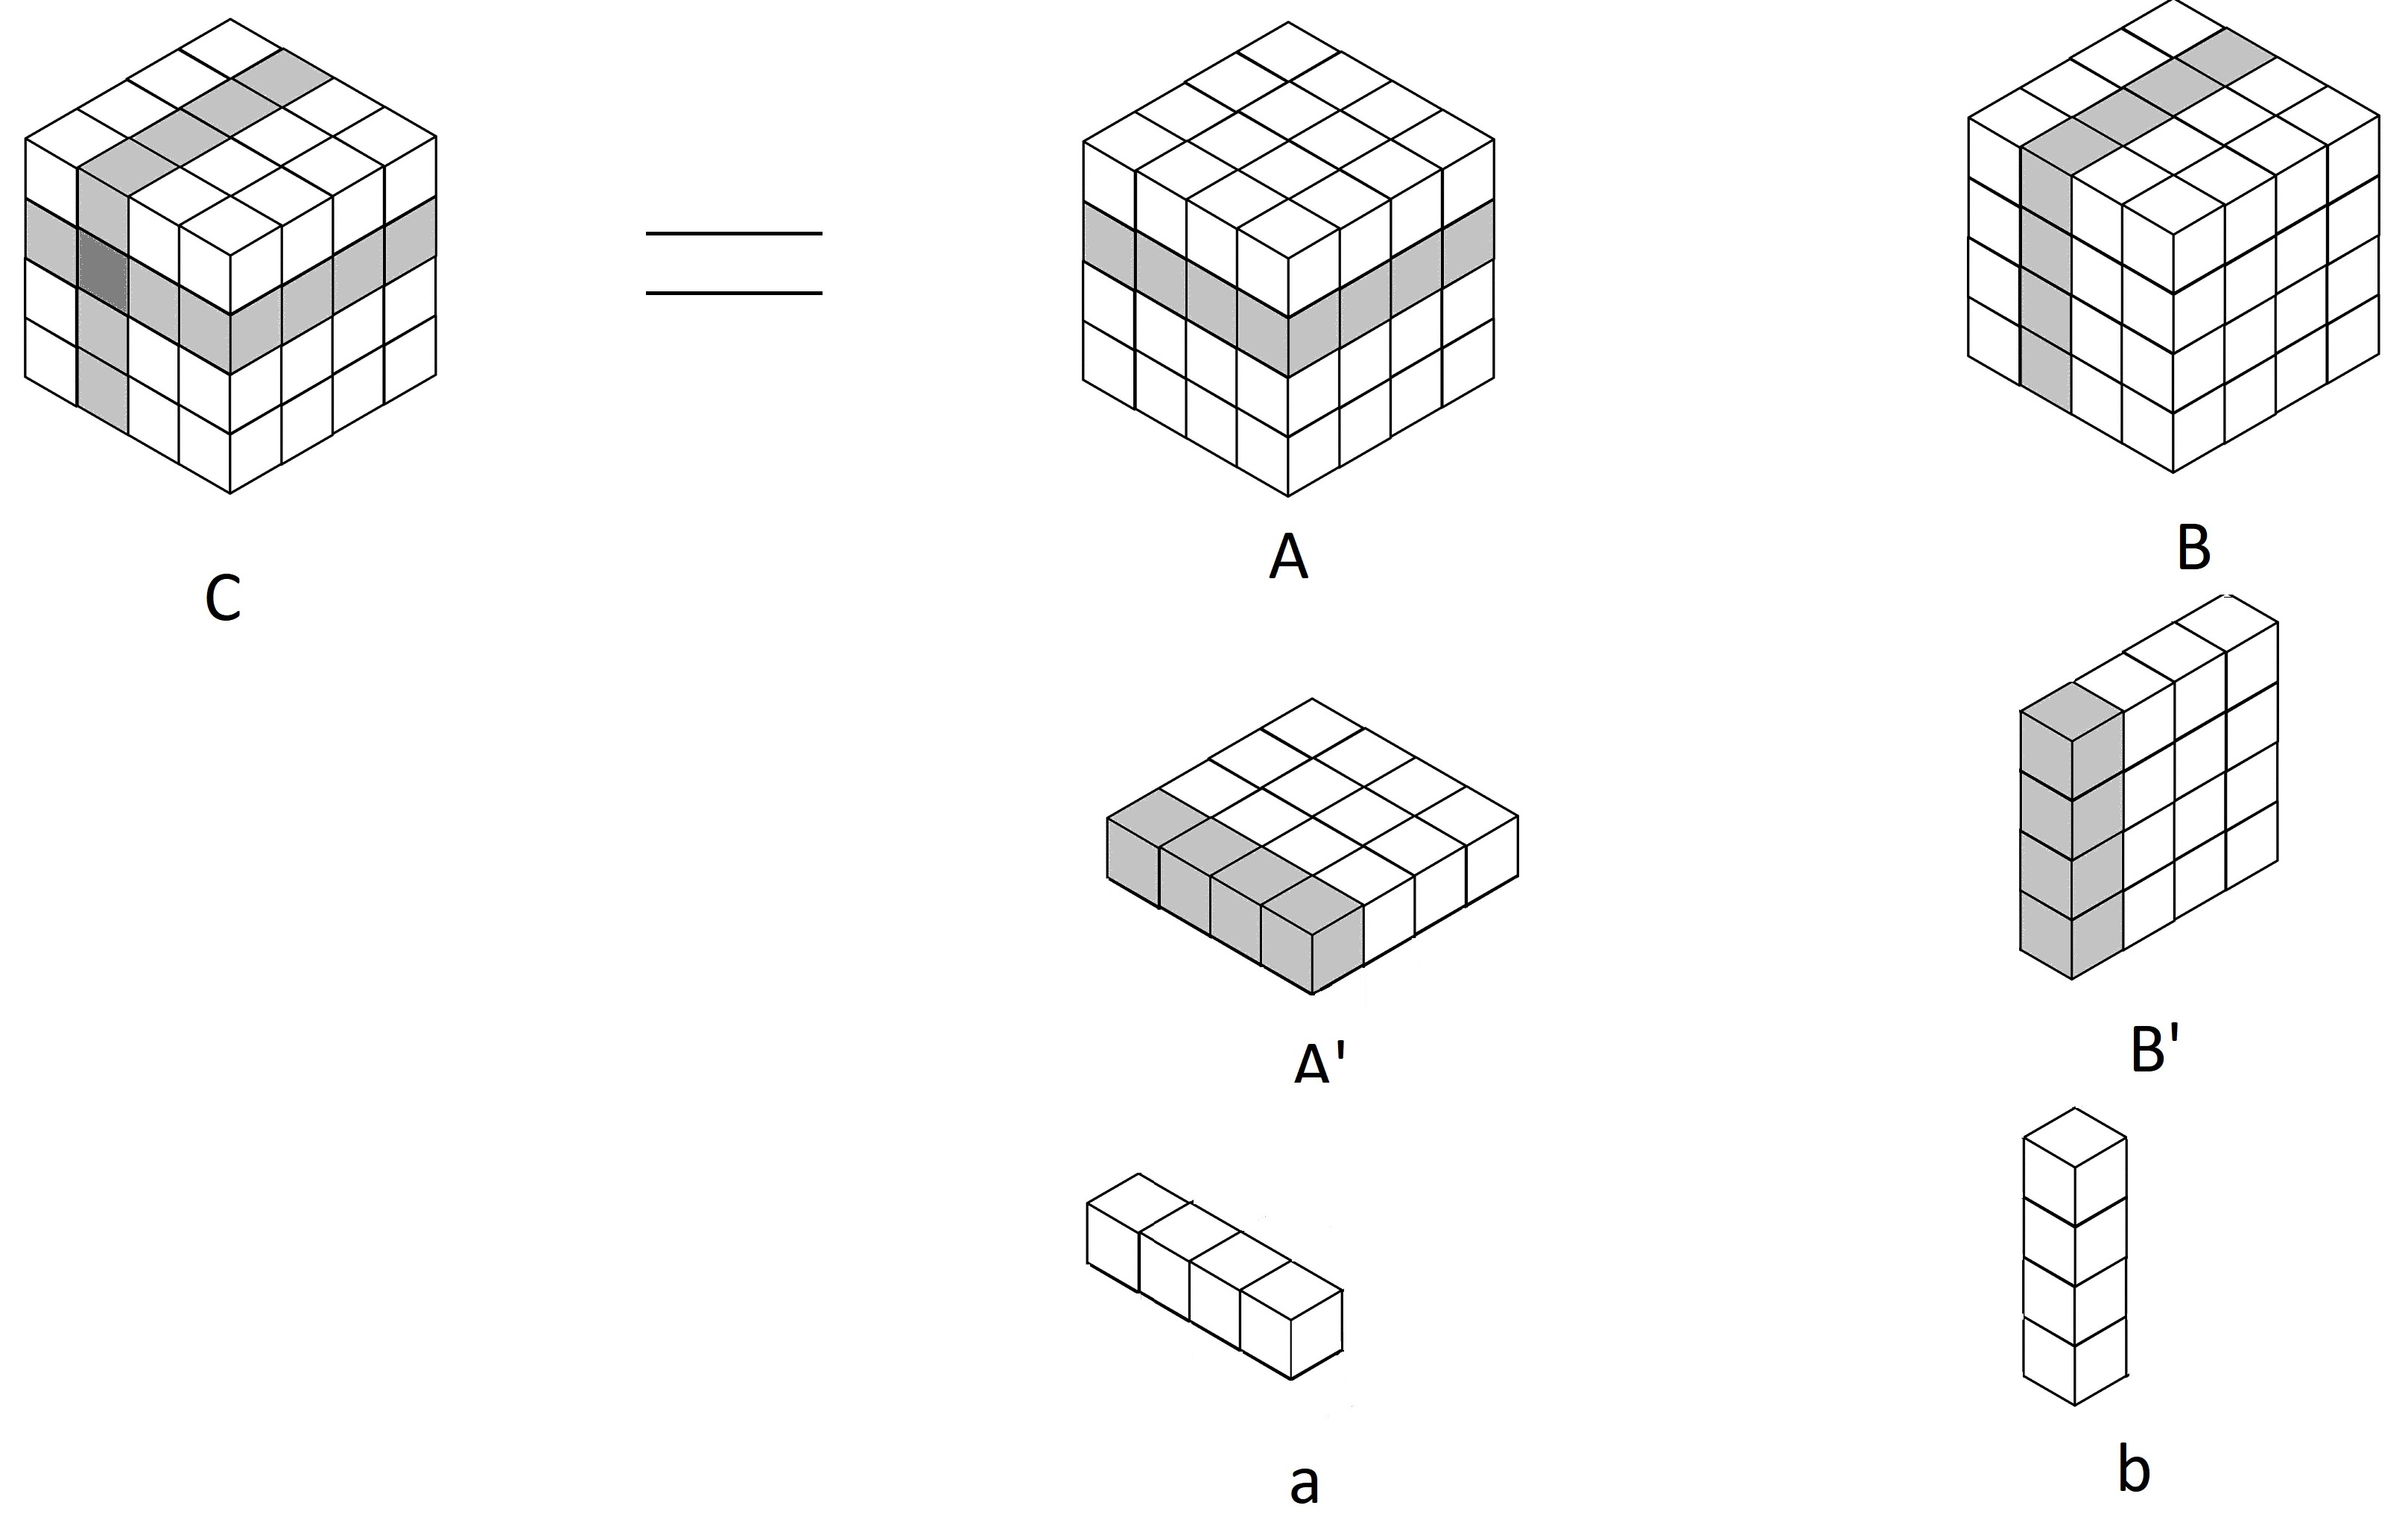
\includegraphics[scale=0.15]{3D.jpg}
\caption{How each element in $C$ was obtained from matrices $A$ and $B$.}\label{3DMult}
\end{figure}

Two \texttt{for} loops were used to maintain the row and column of the current element in matrix $C$.
Another \texttt{for} loop was used to traverse the depth of the matrix $C$.
The row $a$ and column $b$ were then obtained from matrices $A$ and $B$ as seen in figure \ref{3DMult}.
Vector multiplication was then used on vectors $a$ and $b$.
The resulting value is the corresponding element of $C$.

This was repeated for all elements in matrix $C$.

%\begin{algorithm}[H]
%\SetAlgoLined
%\KwData{this text}
%\KwResult{how to write algorithm with \LaTeX2e }
%initialization\;
%\While{not at end of this document}{
%read current\;
%\eIf{understand}{
%go to next section\;
%current section becomes this one\;
%}{
%go back to the beginning of current section\;
%}
%}
%\caption{How to write algorithms}
%\end{algorithm}

\end{document}